\documentclass[tikz,border=14pt]{standalone}
\usepackage[T1]{fontenc}
\usepackage{tgheros}
\usepackage{sfmath}
\usepackage{amsmath}
% % \usepackage{fontawesome5} (Removed for publication-grade academic typography) (Removed for publication-grade academic typography)
\usepackage{tikz}
\usetikzlibrary{arrows.meta,positioning,shapes.geometric,fit,backgrounds,calc}
\usepackage{xcolor}

\renewcommand{\familydefault}{\sfdefault}

% Academic Semantic Palette
\definecolor{harvardcrimson}{HTML}{A51C30}
\definecolor{ethdarkblue}{HTML}{1F407A}
\definecolor{ethblue}{HTML}{215CAF}
\definecolor{ethpetrol}{HTML}{007A87}
\definecolor{ethbronze}{HTML}{B87333}
\definecolor{ethpurple}{HTML}{5B4B8A}
\definecolor{ethslate}{HTML}{475569}
\definecolor{cardbg}{HTML}{F8FAFC}
\definecolor{cardborder}{HTML}{CBD5E1}
\definecolor{safeTeal}{HTML}{10B981}
\definecolor{warnAmber}{HTML}{D97706}
\definecolor{coralRed}{HTML}{DC2626}

\begin{document}
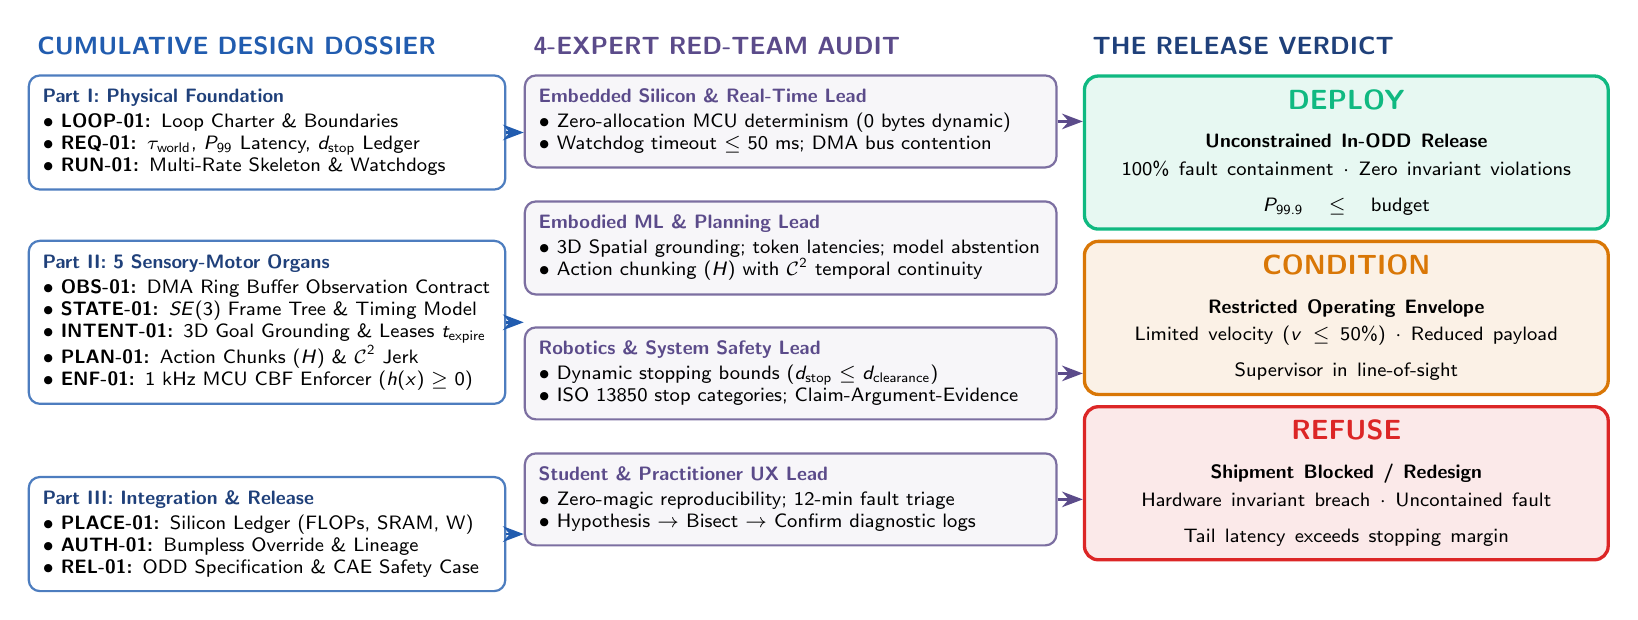
\begin{tikzpicture}[
  font=\sffamily,
  >=Stealth,
  dossierbox/.style={
    draw=ethblue!80,
    fill=white,
    rounded corners=4pt,
    line width=0.8pt,
    inner sep=5pt,
    text width=5.7cm,
    font=\sffamily\scriptsize,
    anchor=north west
  },
  auditbox/.style={
    draw=ethpurple!80,
    fill=ethpurple!5,
    rounded corners=4pt,
    line width=0.8pt,
    inner sep=5pt,
    text width=6.4cm,
    font=\sffamily\scriptsize,
    anchor=north west
  },
  verdictdeploy/.style={
    draw=safeTeal,
    fill=safeTeal!10,
    rounded corners=5pt,
    line width=1.2pt,
    inner sep=5pt,
    text width=6.3cm,
    align=center,
    anchor=north west
  },
  verdictcondition/.style={
    draw=warnAmber,
    fill=warnAmber!10,
    rounded corners=5pt,
    line width=1.2pt,
    inner sep=5pt,
    text width=6.3cm,
    align=center,
    anchor=north west
  },
  verdictrefuse/.style={
    draw=coralRed,
    fill=coralRed!10,
    rounded corners=5pt,
    line width=1.2pt,
    inner sep=5pt,
    text width=6.3cm,
    align=center,
    anchor=north west
  }
]

  % ----------------------------------------------------
  % COLUMN 1: THE 11-ARTIFACT CUMULATIVE DOSSIER
  % ----------------------------------------------------
  \node[font=\sffamily\bfseries\small, text=ethblue, anchor=north west] (c1_hdr) at (0, 8.4) {
     CUMULATIVE DESIGN DOSSIER
  };

  \node[dossierbox] (dossier_p1) at (0, 7.8) {
    \textbf{\color{ethdarkblue}Part I: Physical Foundation}\\[1pt]
    $\bullet$ \textbf{LOOP-01:} Loop Charter \& Boundaries\\
    $\bullet$ \textbf{REQ-01:} $\tau_{\text{world}}$, $P_{99}$ Latency, $d_{\text{stop}}$ Ledger\\
    $\bullet$ \textbf{RUN-01:} Multi-Rate Skeleton \& Watchdogs
  };

  \node[dossierbox] (dossier_p2) at (0, 5.7) {
    \textbf{\color{ethdarkblue}Part II: 5 Sensory-Motor Organs}\\[1pt]
    $\bullet$ \textbf{OBS-01:} DMA Ring Buffer Observation Contract\\
    $\bullet$ \textbf{STATE-01:} $SE(3)$ Frame Tree \& Timing Model\\
    $\bullet$ \textbf{INTENT-01:} 3D Goal Grounding \& Leases $t_{\text{expire}}$\\
    $\bullet$ \textbf{PLAN-01:} Action Chunks ($H$) \& $\mathcal{C}^2$ Jerk\\
    $\bullet$ \textbf{ENF-01:} 1 kHz MCU CBF Enforcer ($h(x) \ge 0$)
  };

  \node[dossierbox] (dossier_p3) at (0, 2.7) {
    \textbf{\color{ethdarkblue}Part III: Integration \& Release}\\[1pt]
    $\bullet$ \textbf{PLACE-01:} Silicon Ledger (FLOPs, SRAM, W)\\
    $\bullet$ \textbf{AUTH-01:} Bumpless Override \& Lineage\\
    $\bullet$ \textbf{REL-01:} ODD Specification \& CAE Safety Case
  };

  % ----------------------------------------------------
  % COLUMN 2: 4-EXPERT RED-TEAM REVIEW BOARD
  % ----------------------------------------------------
  \node[font=\sffamily\bfseries\small, text=ethpurple, anchor=north west] (c2_hdr) at (6.3, 8.4) {
     4-EXPERT RED-TEAM AUDIT
  };

  \node[auditbox] (audit_embed) at (6.3, 7.8) {
    \textbf{\color{ethpurple} Embedded Silicon \& Real-Time Lead}\\[1pt]
    $\bullet$ Zero-allocation MCU determinism ($0\text{ bytes dynamic}$)\\
    $\bullet$ Watchdog timeout $\le 50\text{ ms}$; DMA bus contention
  };

  \node[auditbox] (audit_ml) at (6.3, 6.2) {
    \textbf{\color{ethpurple} Embodied ML \& Planning Lead}\\[1pt]
    $\bullet$ 3D Spatial grounding; token latencies; model abstention\\
    $\bullet$ Action chunking ($H$) with $\mathcal{C}^2$ temporal continuity
  };

  \node[auditbox] (audit_safety) at (6.3, 4.6) {
    \textbf{\color{ethpurple} Robotics \& System Safety Lead}\\[1pt]
    $\bullet$ Dynamic stopping bounds ($d_{\text{stop}} \le d_{\text{clearance}}$)\\
    $\bullet$ ISO 13850 stop categories; Claim-Argument-Evidence
  };

  \node[auditbox] (audit_ux) at (6.3, 3.0) {
    \textbf{\color{ethpurple} Student \& Practitioner UX Lead}\\[1pt]
    $\bullet$ Zero-magic reproducibility; 12-min fault triage\\
    $\bullet$ Hypothesis $\to$ Bisect $\to$ Confirm diagnostic logs
  };

  % ----------------------------------------------------
  % COLUMN 3: THE 3 RELEASE VERDICTS
  % ----------------------------------------------------
  \node[font=\sffamily\bfseries\small, text=ethdarkblue, anchor=north west] (c3_hdr) at (13.4, 8.4) {
     THE RELEASE VERDICT
  };

  \node[verdictdeploy] (v_deploy) at (13.4, 7.8) {
    \textbf{\color{safeTeal} DEPLOY}\\[2pt]
    {\scriptsize \textbf{Unconstrained In-ODD Release}}\\[2pt]
    {\scriptsize $100\%$ fault containment $\cdot$ Zero invariant violations\\[1pt] $P_{99.9} \le \text{budget}$}
  };

  \node[verdictcondition] (v_condition) at (13.4, 5.7) {
    \textbf{\color{warnAmber} CONDITION}\\[2pt]
    {\scriptsize \textbf{Restricted Operating Envelope}}\\[2pt]
    {\scriptsize Limited velocity ($v \le 50\%$) $\cdot$ Reduced payload\\[1pt] Supervisor in line-of-sight}
  };

  \node[verdictrefuse] (v_refuse) at (13.4, 3.6) {
    \textbf{\color{coralRed} REFUSE}\\[2pt]
    {\scriptsize \textbf{Shipment Blocked / Redesign}}\\[2pt]
    {\scriptsize Hardware invariant breach $\cdot$ Uncontained fault\\[1pt] Tail latency exceeds stopping margin}
  };

  % Inter-Column Arrows (strictly horizontal flow)
  \draw[->, line width=1.0pt, ethblue] (dossier_p1.east) -- (dossier_p1.east -| audit_embed.west);
  \draw[->, line width=1.0pt, ethblue] (dossier_p2.east) -- (dossier_p2.east -| audit_safety.west);
  \draw[->, line width=1.0pt, ethblue] (dossier_p3.east) -- (dossier_p3.east -| audit_ux.west);

  \draw[->, line width=1.0pt, ethpurple] (audit_embed.east) -- (audit_embed.east -| v_deploy.west);
  \draw[->, line width=1.0pt, ethpurple] (audit_safety.east) -- (audit_safety.east -| v_condition.west);
  \draw[->, line width=1.0pt, ethpurple] (audit_ux.east) -- (audit_ux.east -| v_refuse.west);

\end{tikzpicture}
\end{document}
